\chapter{Literature Study}
\label{chap:literature}

\npar The mobile industry is without a doubt one of the most vibrant industries at the moment. Not only because mobile device sales are growing rapidly but also because of the highly competitive nature of this market. This has led to fragmentation. 

\npar This chapter will explain the problem of fragmentation and a number of suggested solutions to cope with this problem.

\section{The mobile device landscape}

\npar In the last couple of years, smartphone sales have gone up quickly. Smartphones are becoming ubiquitous and in some regions, like the United States, smartphone penetration has already reached more than 50\% \cite{Nielsen:2012}. According to quarterly studies by Gartner, smartphone penetration remained stable before the iPhone 3G and Android came along (see \fref{fig:smartphone_sales}).

\begin{figure}
    \begin{center}
        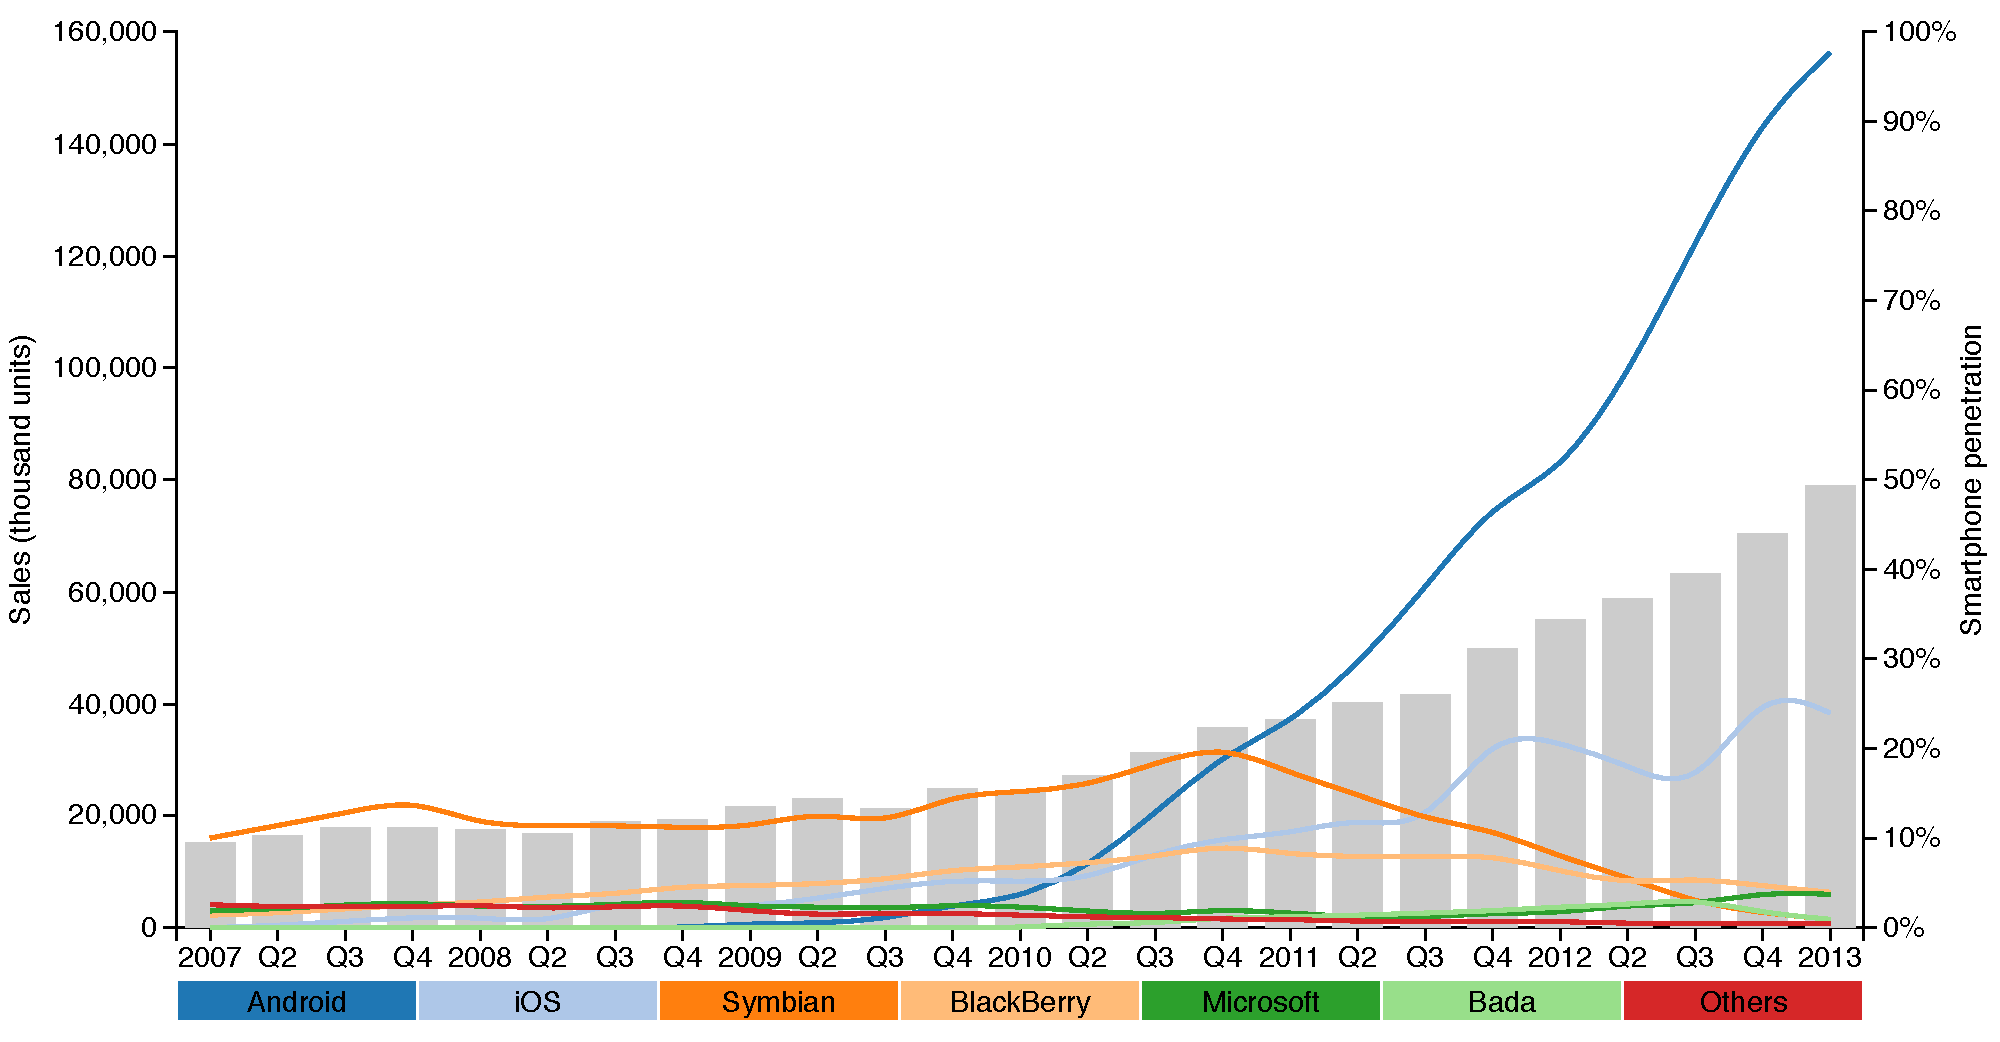
\includegraphics[width=\textwidth]{figs/smartphone_sales.pdf}
        	\caption{
        	    	Growth of worldwide smartphone sales and smartphone penetration. Source: Gartner \citep{Gartner:08Q2,Gartner:08Q3,Gartner:08Q4,Gartner:10Q1,Gartner:10Q2,Gartner:10Q3,Gartner:10Q4,Gartner:11Q1,Gartner:11Q2,Gartner:11Q3,Gartner:11Q4,Gartner:12Q1,Gartner:12Q2}
        	}
        	\label{fig:smartphone_sales}
    \end{center}
\end{figure}

\begin{figure}
    \begin{center}
        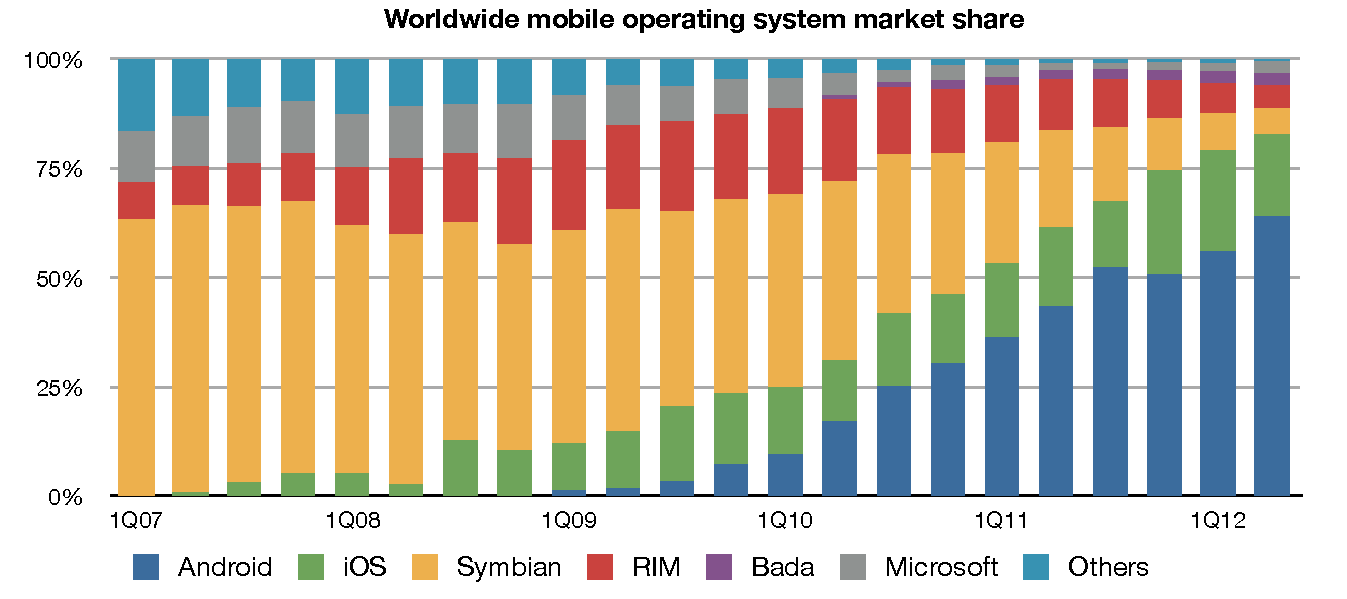
\includegraphics[width=\textwidth]{figs/smartphone_os.pdf}
        \caption{
            Growth of worldwide smartphone operating system market share. Source: Gartner \citep{Gartner:08Q2,Gartner:08Q3,Gartner:08Q4,Gartner:10Q1,Gartner:10Q2,Gartner:10Q3,Gartner:10Q4,Gartner:11Q1,Gartner:11Q2,Gartner:11Q3,Gartner:11Q4,Gartner:12Q1,Gartner:12Q2}
        	}
        \label{fig:smartphone_os}
    \end{center}
\end{figure}

\npar But more importantly, one can conclude that there is not one major platform. Projections by the IDC show that in 2016, there will be at least three major platforms covering 90\% of the worldwide smartphone market \citep{IDC:phone}. 

\npar A similar scenario is playing in the tablet industry. According to other studies by both Gartner \citep{Gartner:11tab,Gartner:12tab} and IDC \citep{IDC:tablet}, tablets will continue to gain popularity and sales will be mainly driven by iPads and Android tablets (see \fref{fig:tablet}).

\begin{figure}
    \begin{center}
        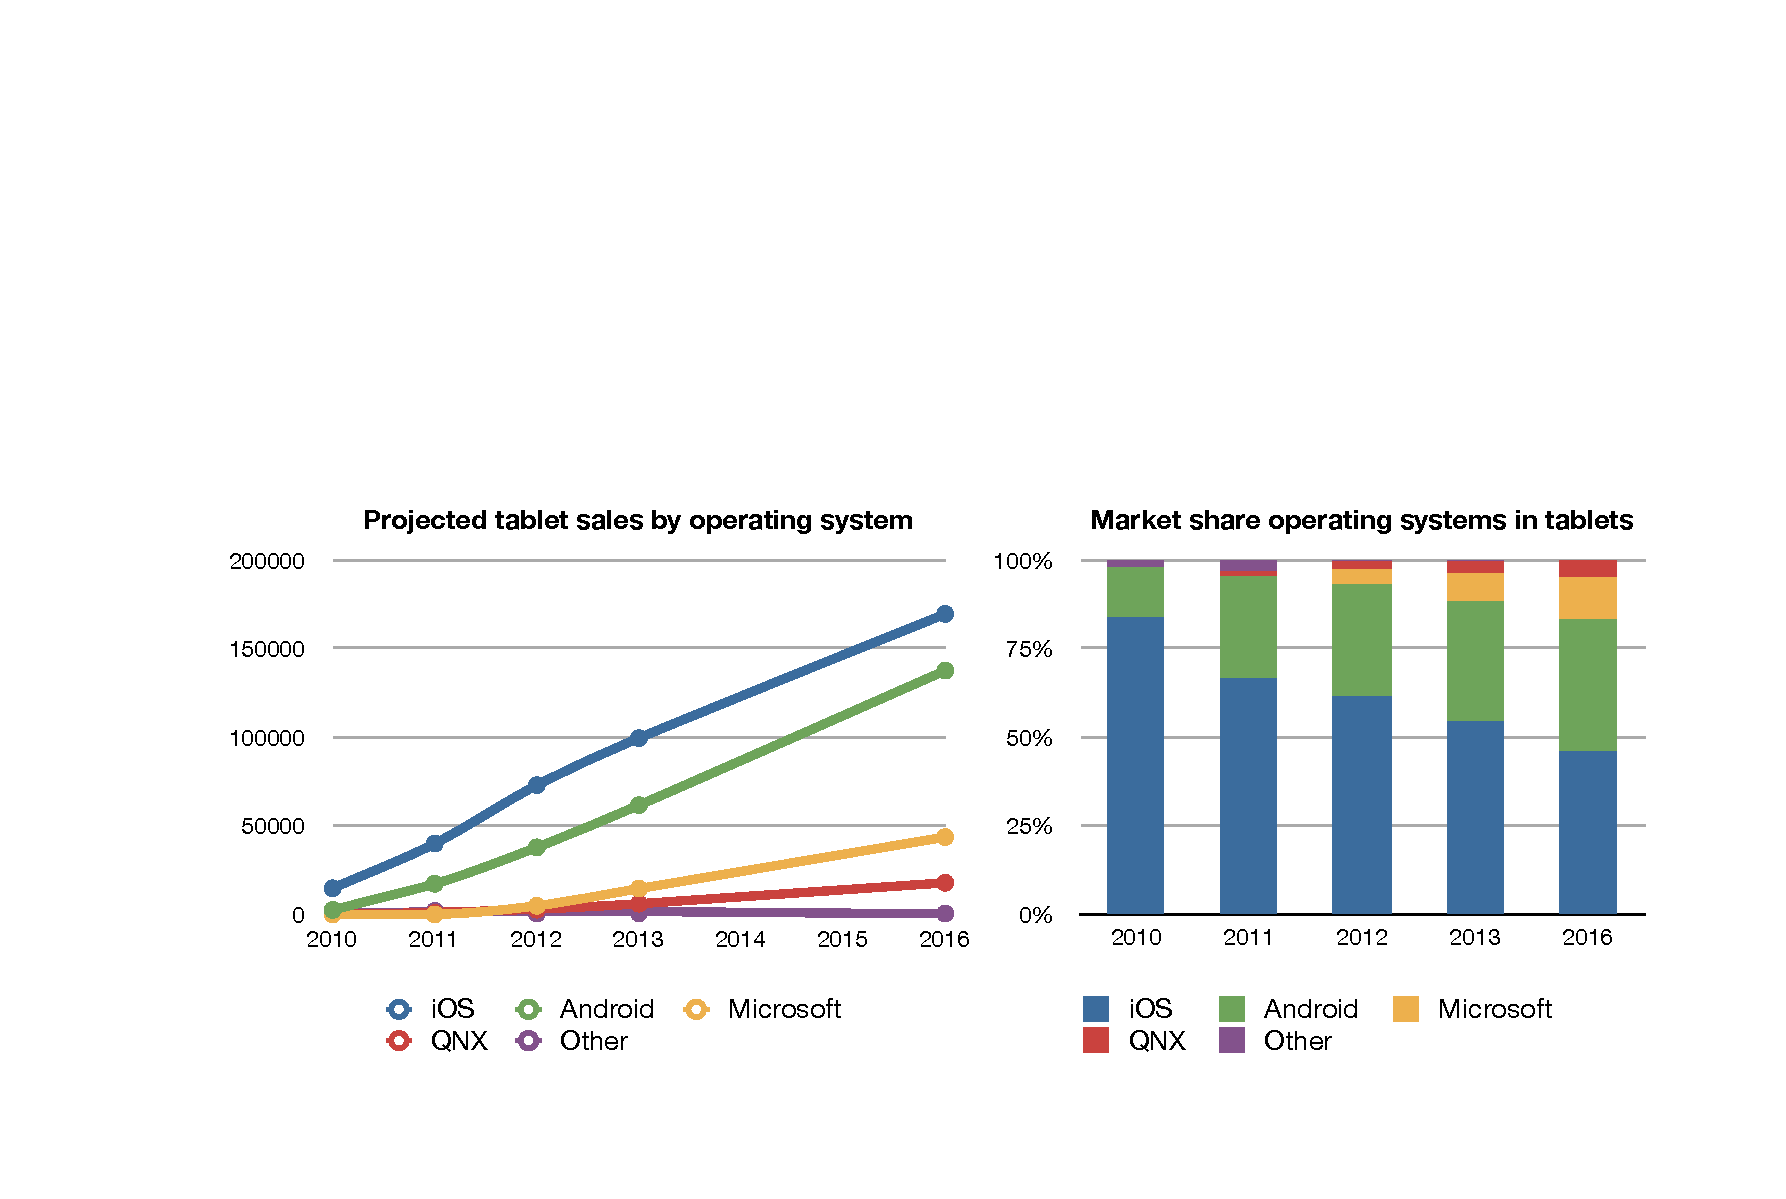
\includegraphics[width=\textwidth]{figs/tablet.pdf}
        \caption{
            Growth of worldwide smartphone sales and smartphone penetration. Source: Gartner \citep{Gartner:11tab,Gartner:12tab}
        }
        \label{fig:tablet}
    \end{center}
\end{figure}

\npar Even though both companies do not agree on which platform will be the biggest by 2016, they both predict there will be at least three major platforms; iOS, Android and Windows. 

% TODO: summary?

\section{The problem of fragmentation}

\npar The competition among mobile device manufacturers has led to fragmentation on many levels. For consumers, fragmentation is usually a good thing. The more different devices there are, the easier it is for a consumer to pick one that fits his needs. For developers on the other hand, fragmentation is usually considered bad. Developers have to develop and test their applications on multiple devices to be able to guarantee the desired experience. This is expensive and time consuming.

\npar From \fref{fig:smartphone_os} and \fref{fig:tablet} it is already clear that the market is divided by operating system or platform but even within these platforms, fragmentation is multi-dimensional \citep{Kindel}.

\npar In general, there are fewer fragmentation problems with Apple's iOS because it is a closed platform. Android, however, is an open source platform and vendors are allowed to tailor it for their devices. As a result, there are hundreds of Android based devices but also hundreds of Android flavours.

\npar Maintenance of such Android flavours is expensive and for this reason, manufacturers do not often provide updates for their devices. This has led to noticeable runtime fragmentation among Android based devices compared to iDevices (see \fref{fig:runtime_fragmentation}). 

\begin{figure}
    \begin{center}
        \label{fig:runtime_fragmentation}
        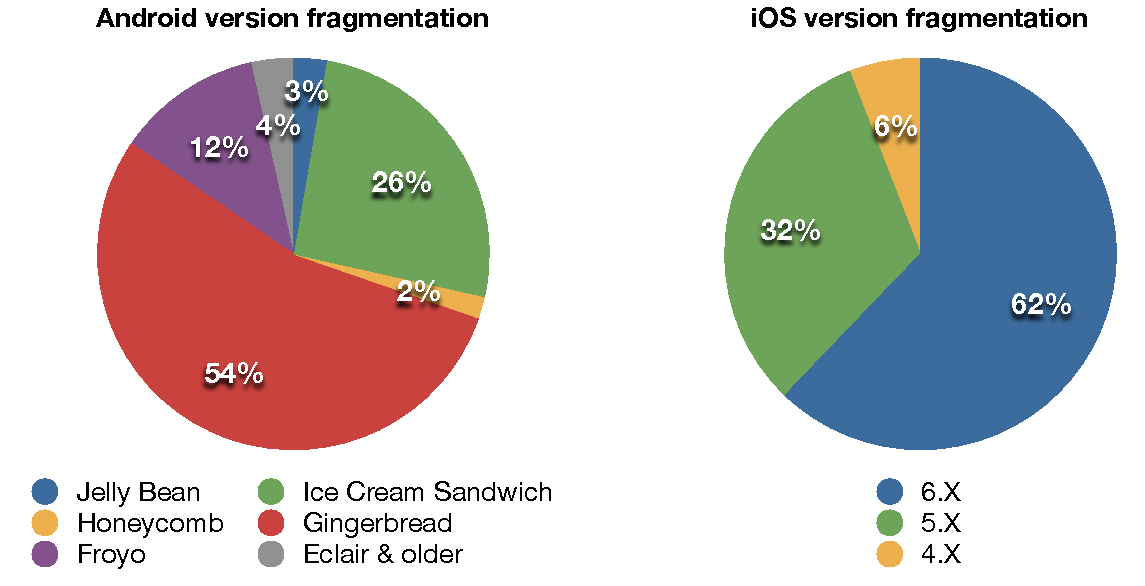
\includegraphics[width=0.8\textwidth]{figs/os_distribution.pdf}
        \caption{
            Runtime fragmentation for Android \citep{android_distribution} and iOS (based on the statistics of developer David Smith) \citep{ios_distribution}.
        }
    \end{center}
\end{figure}

\npar Fragmentation on the device axis is unavoidable but, again, fragmentation among Android based devices is worse than among iDevices. The most relevant items on this axis are the different hardware specifications and screen resolution.

\npar 

\section{Application Architectures}

\npar There are already a number of paradigms for cross platform mobile application development \citep{Friese}. This section presents an overview of the available architectures by comparing different aspects: performance, look and feel, platform access, programming languages, development cost and monetization.

\subsection{Native App}

\npar The default for all applications is a native app. In this paradigm, the application is built for a specific platform and version. Performance of these apps is best and the application will have the look and feel of the platform (providing that no interface elements have been overridden). 

\begin{figure}
    \begin{center}
        %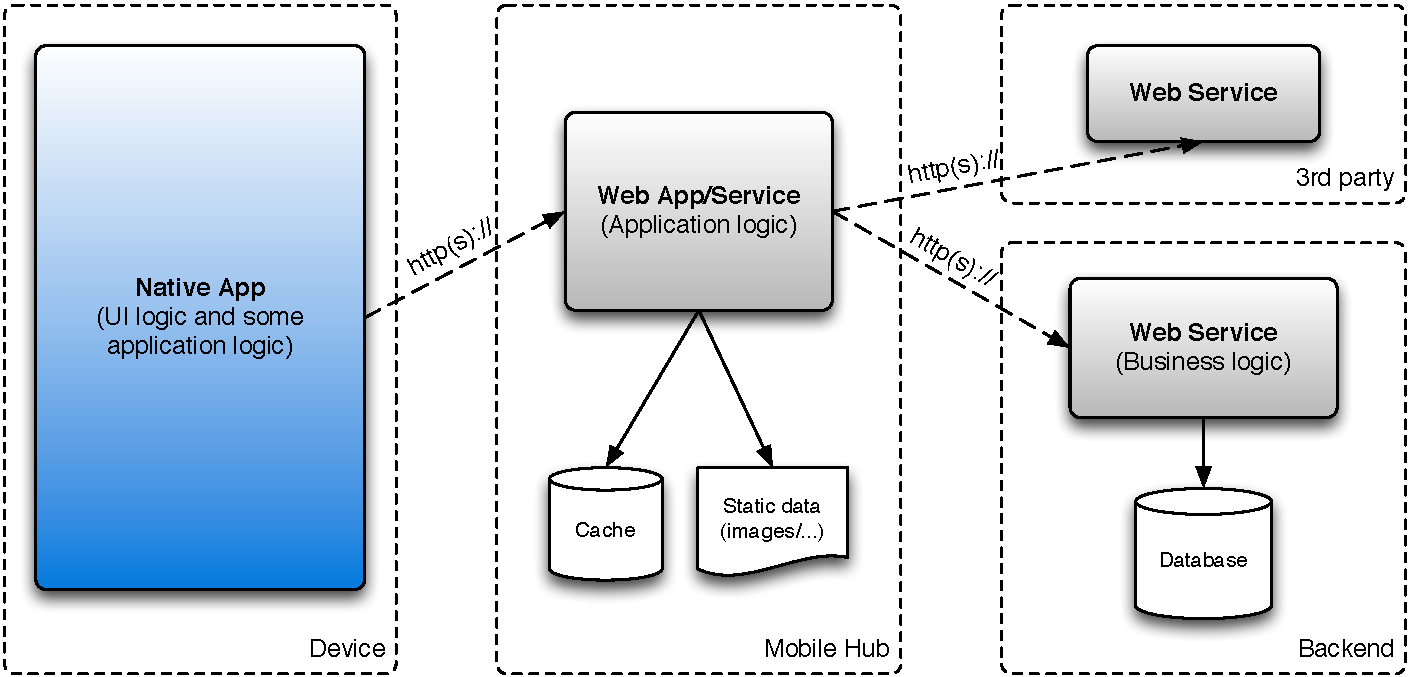
\includegraphics[]{figs/native.pdf}
        \caption{
            Application architecture of a native app, based on \citep{Friese}
        }
        \label{fig:native}
    \end{center}
\end{figure}

\subsection{Web App}

\npar Web apps are web sites that are optimized for mobile browsers. Since every platform comes with a browser, this is the easiest way to get an application running on all platforms. The downside is that mobile web sites lack the capability to access the device (see \fref{fig:web}).

\begin{figure}
    \begin{center}
        %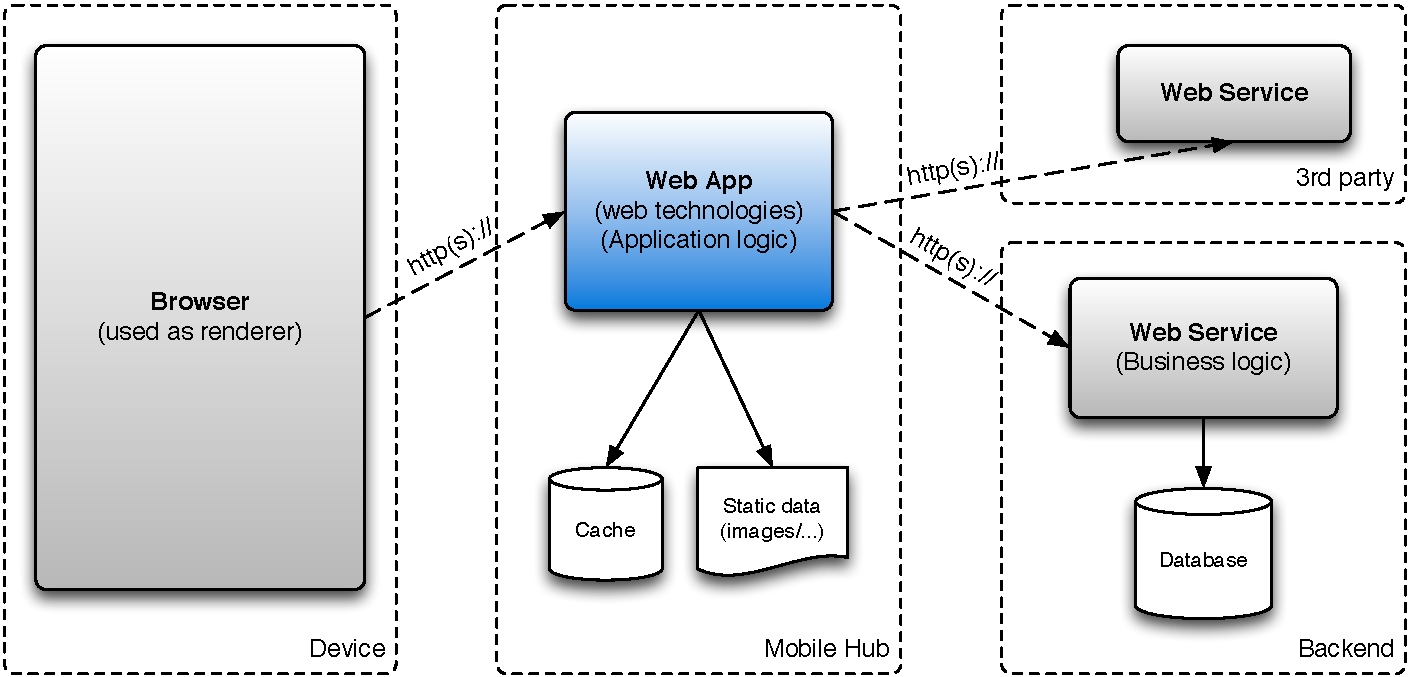
\includegraphics[]{figs/web.pdf}
        \caption{
            Application architecture of a web app, based on \citep{Friese}
        }
        \label{fig:web}
    \end{center}
\end{figure}

\npar With HTML5, web apps can even make use of more powerful features like databases, geolocation, etc. The only barrier for now is the incomplete HTML5 support on mobile browsers.

\subsection{Hybrid App}

\npar Hybrid applications are the logical next step, combining native apps and web apps. The actual application is a web site, wrapped in a web view, part of a native shell. Except for the name and some specific extensions, this shell can be reused. Platform access is provided through a bridge (see \fref{fig:hybrid}). 

\begin{figure}
    \begin{center}
        %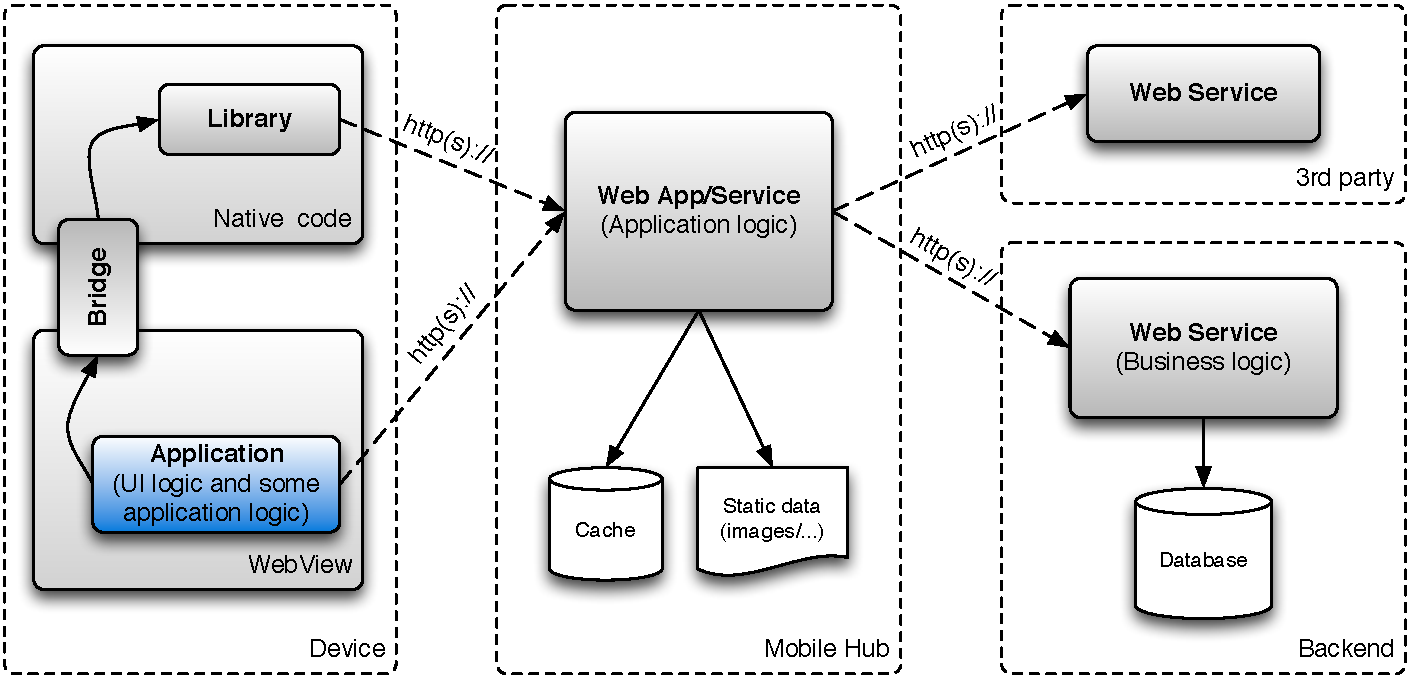
\includegraphics[]{figs/hybrid.pdf}
        \caption{
            Application architecture of a hybrid app, based on \citep{Friese}
        }
        \label{fig:hybrid}
    \end{center}
\end{figure}

\npar

\subsection{Interpreted App}

\npar In an interpreted application, instructions are translated to native instructions at runtime.

\begin{figure}
    \begin{center}
        %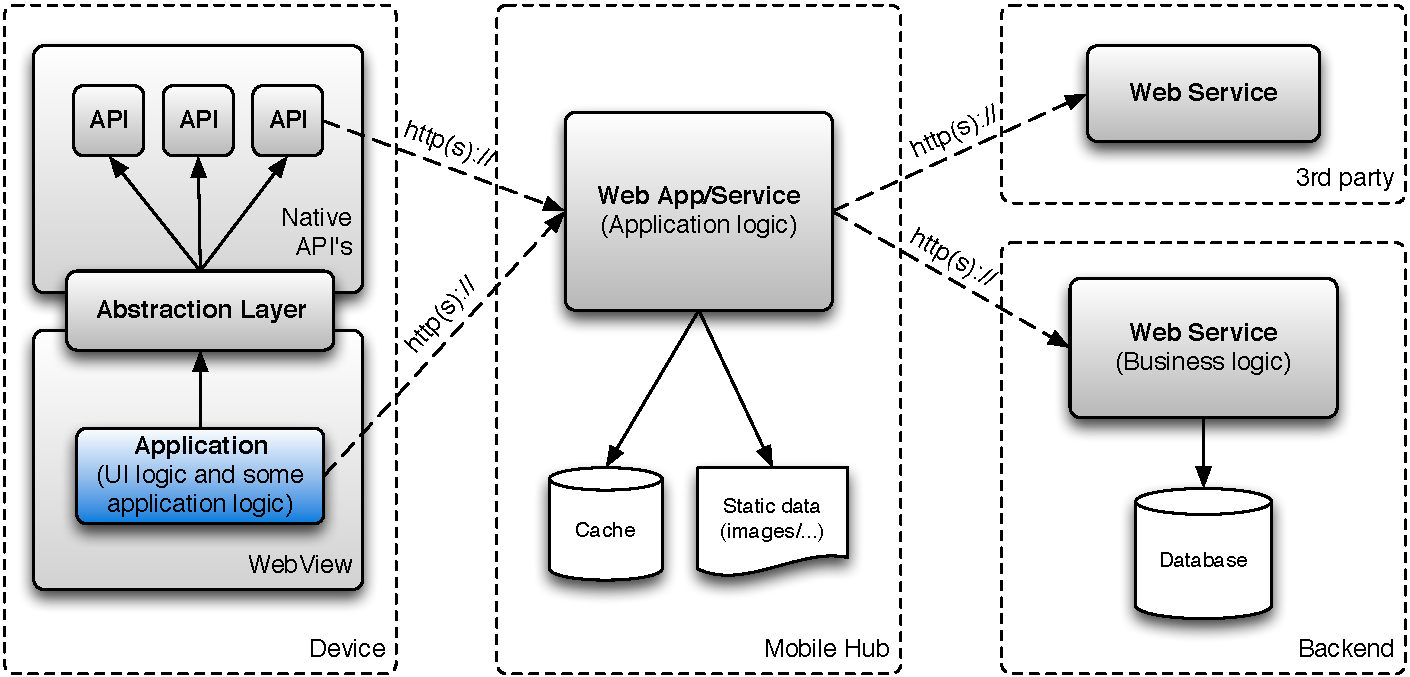
\includegraphics[]{figs/interpreted.pdf}
        \caption{
            Application architecture of an interpreted app, based on \citep{Friese}
        }
        \label{fig:interpreted}
    \end{center}
\end{figure}

\subsection{Cross Compiling}

\npar Instead of translating instructions at runtime, one can translate instructions at compile time. The process is called cross compiling and the result is a truly native app. Performance is similar to native apps but 

\begin{figure}
    \begin{center}
        %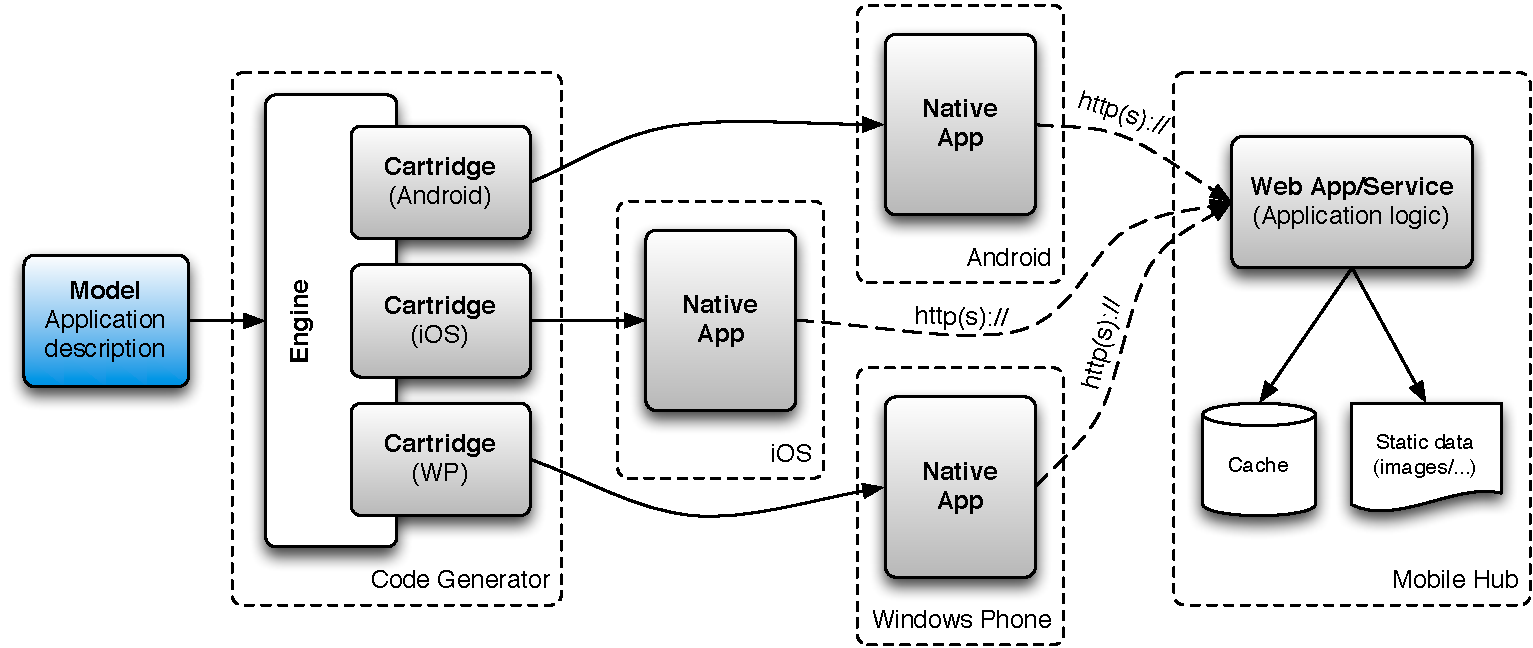
\includegraphics[]{figs/crosscompiled.pdf}
        \caption{
            Architecture used to create cross compiled apps, based on \citep{Friese}
        }
        \label{fig:crosscompiled}
    \end{center}
\end{figure}

\subsection{Summary}

\begin{table}
    \begin{center}
        \begin{tabular}{l|c|c|c|c|c}
                         & Native App & Web App & Hybrid App & Interpreted App & Cross Compiling\\\hline
            Performance  &            &         &            &                 &                \\
            Look \& Feel &            &         &            &                 &                \\
            Distribution &            &         &            &                 &                \\
        \end{tabular}
		\caption{
			Summary of cross platform mobile application development strategies
		}
		\label{tab:architectures}
    \end{center}
\end{table}

\npar

\section{Reflection}

\section{Conclusion}